\chapter{Introduction}
In this document we will elaborate on the design decisions and other considerations in making our videogame ``Crouching Zombie Hidden Viking''. The game include aspects from Computer Graphics (CG) and some from Artificial Intelligence (AI). Because there was particularly little experience with AI in our group we decided, in consultation with our tutor, to focus mainly on the CG challenges of our game.

\section{Game description}
After considering various genres of videogames we decided on strategy as the preferred genre for our game. This would allow for interesting Artificial Intelligence implementations and seemed generally fun. To include the varying levels of intelligence, enemy variety came to mind. The past few years there has been a trend in videogames producing a myriad of different zombie themed games which featured significant enemy variety. Our concept will combine post-apocalyptic zombie game  elements with the real time strategy genre.

During the conceptualisation phase we came up with the slightly humorous ``Crouching Zombie Hidden Viking'' as a name for our game. The player will control a group of organized post-apocalyptic survivors calling themselves vikings in an attempt to rid the world of the numerous zombies. The vikings will have to gain strength though by gathering resources, men and by staying alive in the process.

An important theme in our game is light. The world in itself contains almost no light sources. Most of the world is completely blacked out. Vikings can place and carry light sources like torches. This will help the player in a couple of ways: he can see the direct surroundings, and the zombies get slowed down in the light.

\begin{figure}[!htb]
	\centering
	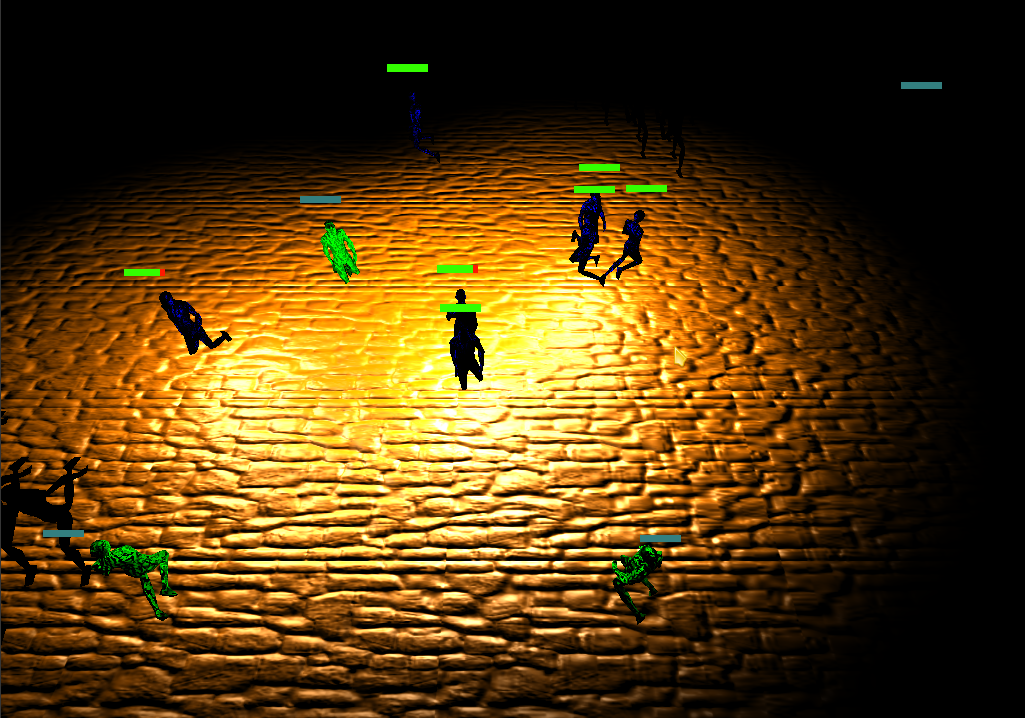
\includegraphics[width=\textwidth]{czhv.png}
	\caption{An impression of what Crouching Zombie Hidden Viking looks like.}
\end{figure}

\FloatBarrier